\documentclass{article}

\usepackage{amsmath, amsthm, amssymb} %Typical Math-packages
\usepackage{enumerate}
\usepackage{graphicx}

\title{The Mathematics Behind Computer Graphics}
\author{Tom Bannink \and Jan-Willem Buurlage}
\date{}
\begin{document}
\maketitle

In this document we will give an introduction to the mathematics behind computer graphics. We will first discuss the basic matrices involved, and how one can compute them. Then we will touch on the subject of lightning, and also dicuss a technique called shadowmapping.

\section{Rendering 3D-objects on a 2D-screen}

The first problem that arises is how to render a three-dimensional world on a computer screen. Consider for a moment the field of view of an eye, or camera - located at the origin, looking at $z^+$. 

\begin{figure}[h!]
	\begin{center}
	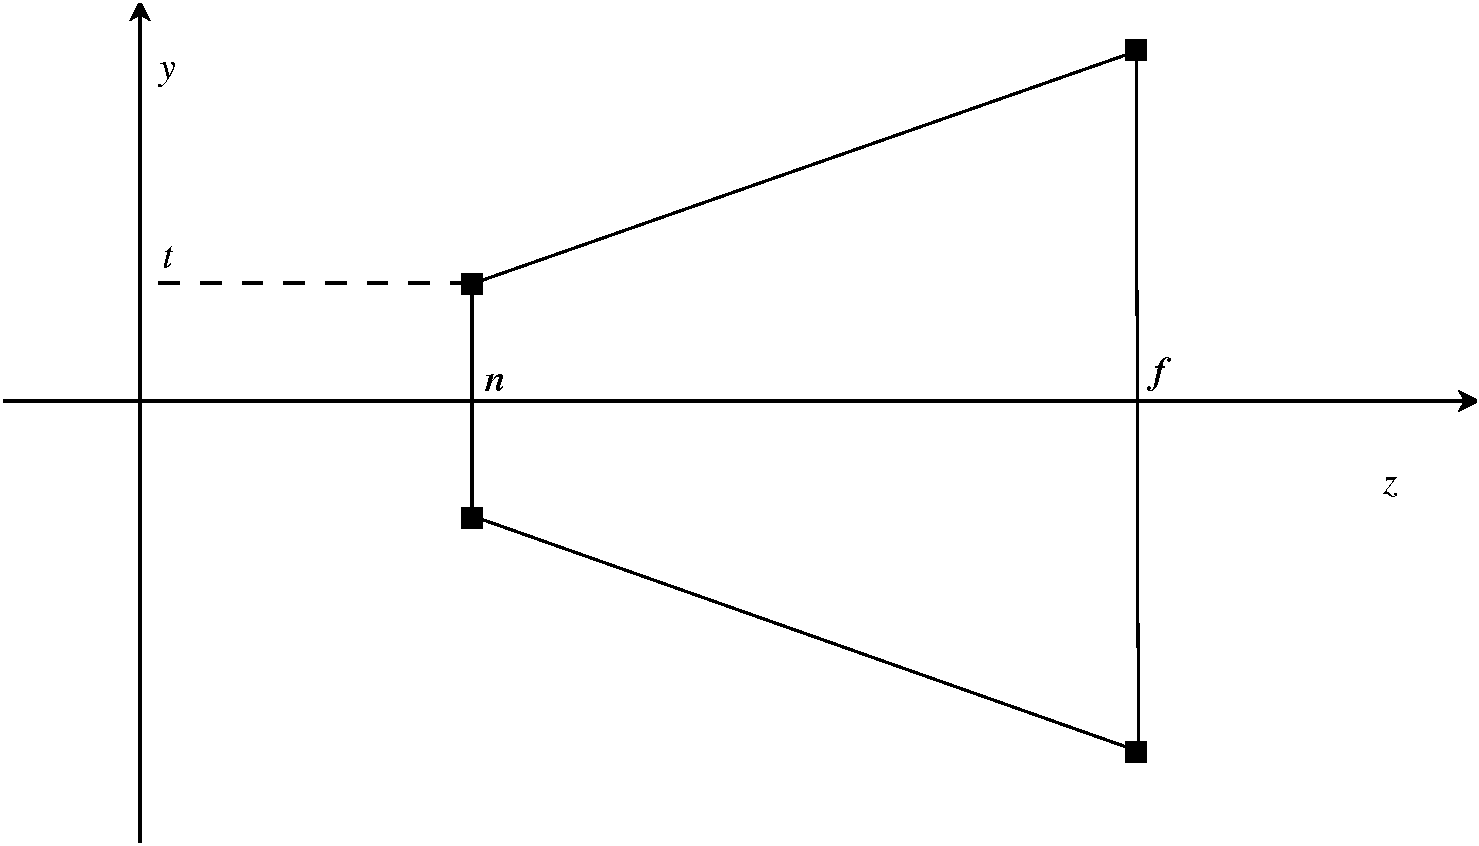
\includegraphics[width=0.8 \textwidth]{frustum-z-y.pdf}
	\caption{Our field of view along the z,y-axes. This extends naturally to a similar image for z,x}
	\end{center}
\end{figure}

We will call the \emph{minimum distance} for which we can view things $n$, and the \emph{maximum distance} we will call $f$. We will denote these planes, parallel to the $z$-axis with the \emph{near} and \emph{far} planes respectively. The width and height of the near plane will be denoted with $2r$ and $2t$ respectively. 

We want to map (we will call this map $P$, from \emph{projection}) this region of space $E$ (eye), into the unit cube $[-1, 1]^3$, for which we'll write $C$ (cube). To do this we will first map the $x$ and $y$ coordinate to the near plane ($N$). Let us denote a point in $E$ with $(x, y, z)$, the corresponding point on $N$ with $(x_N, y_N)$ and the final image in $C$ with $(x', y', z')$. How do we find $x_N, y_N$? We will use similar triangles (see figure). We find:

\begin{align*}
	\frac{n}{z} = \frac{x_N}{x} &\implies x_N = \frac{n}{z_E} x\\	 
	\frac{n}{z} = \frac{y_N}{y} &\implies y_N = \frac{n}{z_E} y
\end{align*}

Mapping $N$ to $C$ is easier, since we know:

\begin{align*}
	[-r, r] \mapsto [-1, 1] \text{ for } x_N &\implies x' \mapsto \frac{x_N}{r} \\
 [-t, t] \mapsto [-1, 1] \text{ for } y_N &\implies y' \mapsto \frac{y_N}{t}
\end{align*}

Once again, the easiest way to see this is by looking at the figure. Combining both equations gives us:

$$x' = \frac{n}{z r} x; \hspace{0.5 cm} y' = \frac{n}{z t} y$$

Note that while $x'$ and $y'$ aren't linear in $x$ and $y$ respectively, $x'z$ and $y'z$ are. Therefore we will introduce homogenous coordinates, and search for $z'z$.

So we want to write $z'z = a \cdot z + b$, because it shouldnt depend on $x$ or $y$. We have the pairs $(z', z) = (-1, n)$ and $(1, f)$. This leads to $a = \frac{f+n}{f-n}$ and $b = -n -n \frac{f+n}{f-n}$. Because $w' = 1$, we have $w'z = z$. We are now ready to find a map $P$ such that $P \cdot \vec{x} = \vec{x'}z$. We can simply read the coefficients for our matrix directly from our equations, because they're all linear. 

$$\begin{pmatrix} x'z\\y'z\\z'z\\w'z \end{pmatrix} = \begin{pmatrix} \frac{n}{r} x\\\frac{n}{t} y\\\frac{f+n}{f-n}z - n(1 + \frac{f+n}{f-n})\\z \end{pmatrix}$$

So for our projection matrix $P$ we have

$$\begin{pmatrix} \frac{n}{r}&0&0&0 \\ 0&\frac{n}{t}&0&0 \\ 0&0&\frac{f+n}{f-n}&- n(1 + \frac{f+n}{f-n}) \\ 0&0&1&0 \end{pmatrix} \begin{pmatrix} x\\y\\z\\1 \end{pmatrix} = \begin{pmatrix} x'z\\y'z\\z'z\\w'z \end{pmatrix}$$

Because $w'z = z$, we can divide by the last coordinate to get $(x', y', z', 1)$ and we're done.

\section{Lightning}

\section{Shadows}



\end{document}